\section{연구 과정}

\subsection{GS-touch 하드웨어 제작}

\subsubsection{사용한 부품}


천체망원경 모터 초점 조절 장치 컨트롤러를 제작하기 위해서 필요한 부품들을 선정하였다. Fig. \ref{fig:parts}은 주요 부품들의 모습이고, 모든 부품의 스펙(specifications)을 아래에 정리하였다. 

\begin{figure}[h]
	\begin{center}
	\begin{tikzpicture}
	\node[anchor=south west,inner sep=0] at (0,0) {
		{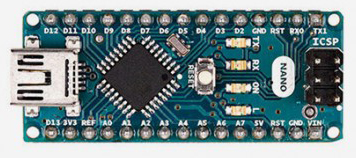
\includegraphics[width = 5.5cm]{arduino_nano-1}} 
		{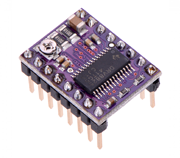
\includegraphics[width = 3.5cm]{DRV8825-1}}
		{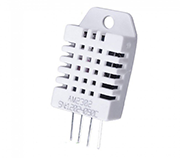
\includegraphics[width = 3.5cm]{DHT22-1}}
		{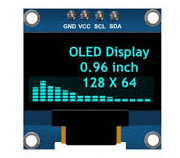
\includegraphics[width = 3.5cm]{OLED-1}} };
	\draw (0.5, 2.6) node {(a)};
	\draw (6.0, 2.6) node {(b)};
	\draw (10.0, 2.6) node {(c)};
	\draw (12.8, 2.6) node {(d)};
	\end{tikzpicture}
	\end{center}
	\caption{GS-touch 제작에 사용된 주요 부품들: (a) Arduino nano, (b) DRV8825, (c) DHT22, (d) OLED displayer.}
	\label{fig:parts}
\end{figure}

\begin{description}[font=$\bullet$~\normalfont\scshape\color{red!50!black}]
	\item [ARDUINO NANO] 모터 초점 조절 장치 컨트롤러를 만드는 데 있어 가장 중요한 부품으로, 일종의 작은 컴퓨터와 같은 역할을 한다. Arduino는 마이크로 컨트롤러를 달고 있는 기판으로, Arduino의 여러 가지 핀에 전선을 연결한 뒤에 코딩하여 Arduino에 올리면 Arduino가 코딩된 내용을 그대로 실행할 수 있도록 하는 hardware이다. 내부에 컴퓨터 역할을 하는 MPU인 ATmega328가 탑재되어 있으며, 5V를 공급할 시에 작동한다. 크기는 45mm x 18mm이다.
	\item [DRV8825] 스테핑 모터를 돌리는 데 있어서 전류를 쉽게 조절할 수 있게 해주는 module이다. 이뿐만이 아니라 모터를 좀 더 세밀하게 돌릴 수 있게 해주는(스텝 당 돌아가는 각도를 줄여주는) 마이크로 스텝을 구현 가능한데, DRV8825의 핀 중 M1, M2, M3의 up, down을 조절하여 full step을 원래 각도와 비교하면 얼마나 적게 돌릴 것인지 결정할 수 있게 한다. 본 모델은 최대 1/32까지의 마이크로 스텝이 가능하다.
	\item [DHT22] 온도와 습도를 측정할 수 있는 감지기로, -40~80℃의 넓은 온도 측정범위와 약 0.5℃밖에 없는 오차를 가지고 있다. 이를 통해 온도나, 렌즈의 온도 상태를 볼 수 있으며, 이를 사용하면 좀 더 정밀한 측정이 가능할 것이다.
	\item [0.96" oled screen I2C] Arduino와 I2C 방법으로 통신을 할 수 있는 OLED 디스플레이어이다. 여러 가지 정보가 전달되며, 모터를 얼마나 돌릴 것인지, 혹은 얼마나 돌려져 있는지 등이 표현될 수 있다.
	\item [Apem MJTP1230B 버튼스위치] 누르는 버튼의 일종으로, 다리가 4개 달린 상태에서 같은 방향에 있는 2개의 전선이 연결된 방식의 버튼이다. 내부의 pull-up 저항을 활용하면 Arduino와 직접 연결하는 것으로 작동시킬 수 있다.
	\item [BP5277-90] 모터를 돌리기 위해서는 12V의 전압이 필요하다. 즉, 12V의 전압을 이용하여 모터를 돌리면서 Arduino를 실행시키기 위해서는 12V를 Arduino의 입력전압인 5V까지 낮출 필요가 있다. 이에 regulator와 축전기를 활용하여 가장 안전하게 5V까지 전압을 낮출 수 있는 regulator를 선택하였다.
	\item [HC-06 bluetooth] 무선통신 장치이다. 여러 가지 무선통신 장치 중에서 블루투스 module의 역할을 하고 있다.
	\item [LED 3mm 90$\deg$, Ohmite OD473JE] 전원이 여러 개가 존재할 수 있으므로, 모터가 돌아갈 수 있는 전압인 12V의 외부전압이 들어왔을 때만 LED가 깜빡일 수 있게 하여 모터가 돌아갈 수 있는 전압이 되었는지 확인할 수 있도록 하는 역할을 하고 있다.
	\item [Panasonic EEA-GA1C100H] 모터를 돌리는 상황에서 큰 전류를 사용하기 때문에 전류가 역방향으로 흐르는 등의 문제를 방지하기 위하여 100μF의 축전기를 사용하였다.
	\item [SparkFun WRL-13678 (ESP8266, ESP01)] 무선통신 장치이다. 여러 가지 무선통신 장치 중에서 WIFI 모듈을 담당한다. 입력전압이 5V가 아닌 3.3V이다.
	\item [Sprague 1C10X7R104K050B] 부품별로 각각 연결된 축전기로, 모두 같은 전압 차를 가지고 있지만, 전류의 noise filtering을 하는 역할로, 필수적으로 사용되었다.

	\item [TE Connectivity/AMP 5525258-3 및 Wurth Elektronik 694106301002] 12V 외부 전원과 모터를 연결하는 선을 연결할 수 있게 하는 module이다.
\end{description}

\clearpage
\subsubsection{프로토타입(Prototype) 기판 제작}

주어진 부품들을 하나 하나 연결하여 만능기판에 와이어로 납땜을 하여 Fig. \ref{fig:prototype}\과 같은 프로토 타입(prototype) 회로를 제작하였다. 각 부품을 사용할 때에는 각 부품의 동작 전압, 허용 전류와 같은 여러 가지 스펙들을 생각하여 회로를 구성해야 한다. 예를 들어 WIFI 모듈인 ESP8266과 같은 경우 그 동작 전압이 5V가 아닌 3.3V이기 때문에 주의하여야 한다. 또한, 각 부품 별로 제조사의 data sheet를 참조하여 여러 가지 문제점들을 미리 방지하였다. 일부 부품은 극성에 유의해야 하며, 

특히 5V를 3.3V로 바꾸는 과정에서는 전압 나눔 회로를 이용하여 전압을 나눌 수 있으나, 12V를 5V로 바꾸는 과정에서는 충분한 전류를 확보하기 위하여 LM7805 regulator를 사용하였다. 부품의 갯수가 많아지면서 배선을 하는데 어려움이 있었지만 회로가 정상적으로 동작하는 것을 확인할 수 있었고, 모터 회전, OLED 디스플레이, 시리얼 통신 등의 코드를 연습할 수 있었다.

\begin{figure}[h]
	\begin{center}
		\begin{tikzpicture}
		\node[anchor=south west,inner sep=0] at (0,0) 
		{
			{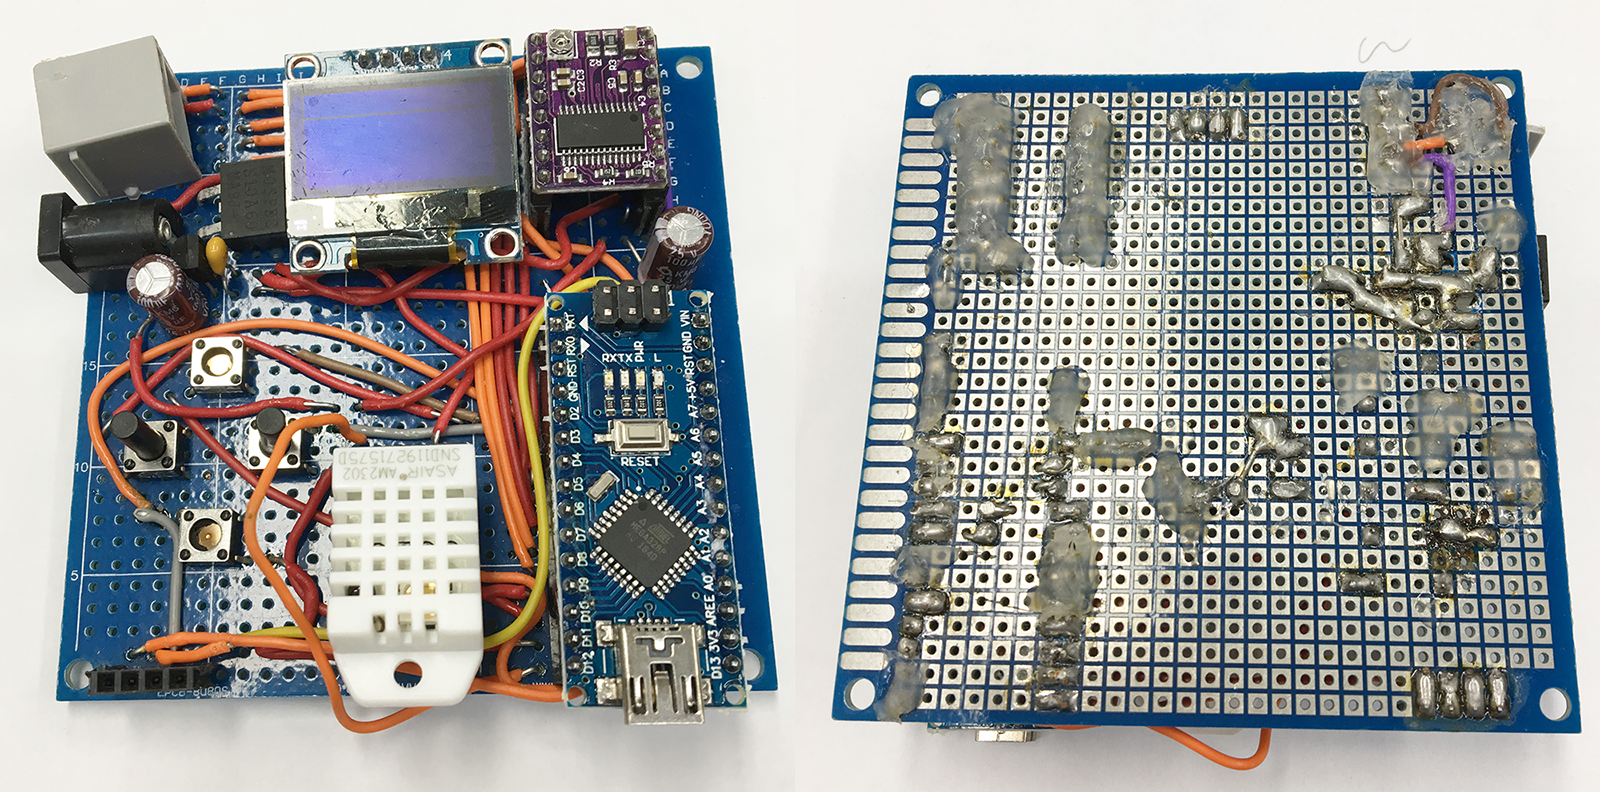
\includegraphics[width=0.7\linewidth]{prototype}} 
		};
		\draw (0.3, 5.4) node {(a)};
		\draw (6.1, 5.4) node {(b)};
		\end{tikzpicture}
		\caption{만능 기판으로 제작한 프로토타입 하드웨어 (a) 앞면과 (b) 뒷면}
		\label{fig:prototype}
	\end{center}
\end{figure}

\subsubsection{회로도 작성 및 PCB 제작}

연구 초반에는 Arduino와 직접 연동이 가능한 Fritzing (https://fritzing.org/home/)을 사용하였지만, 연구가 진행될수록 다른 부품들과 실제로 구현이 가능한 PCB 회로기판을 만들기 위해서 무료로 사용 가능한 PCB 회로 제작 프로그램이면서 협업 기능을 사용할 수 있는 Circuit maker (https://circuitmaker.com/)를 사용하게 되었다. 

\begin{figure}[h]
	\begin{center}
		\begin{tikzpicture}
		\node[anchor=south west,inner sep=0] at (0,0) 
		{
			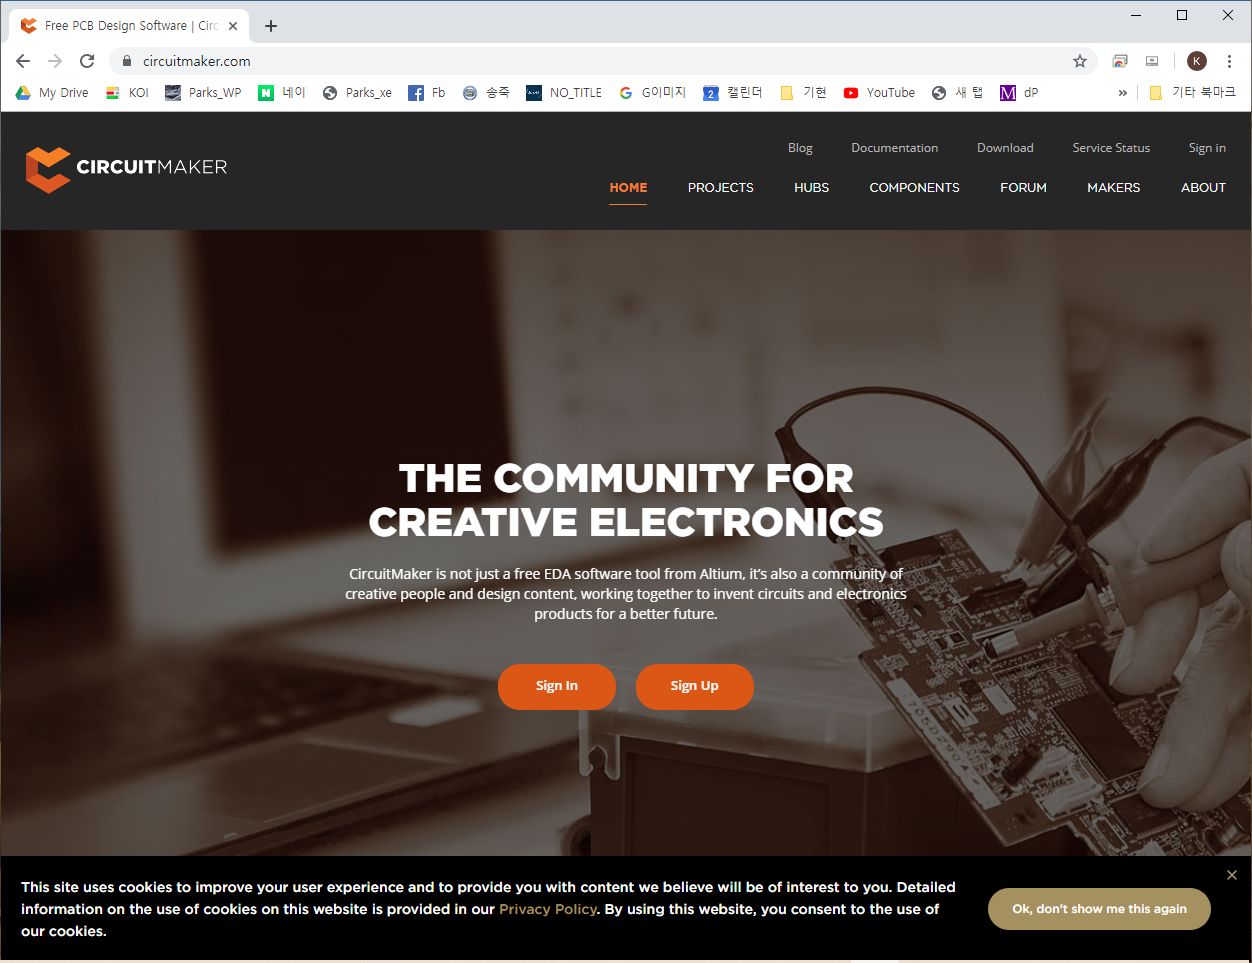
\includegraphics[width=0.42\linewidth]{circuit_maker2}
			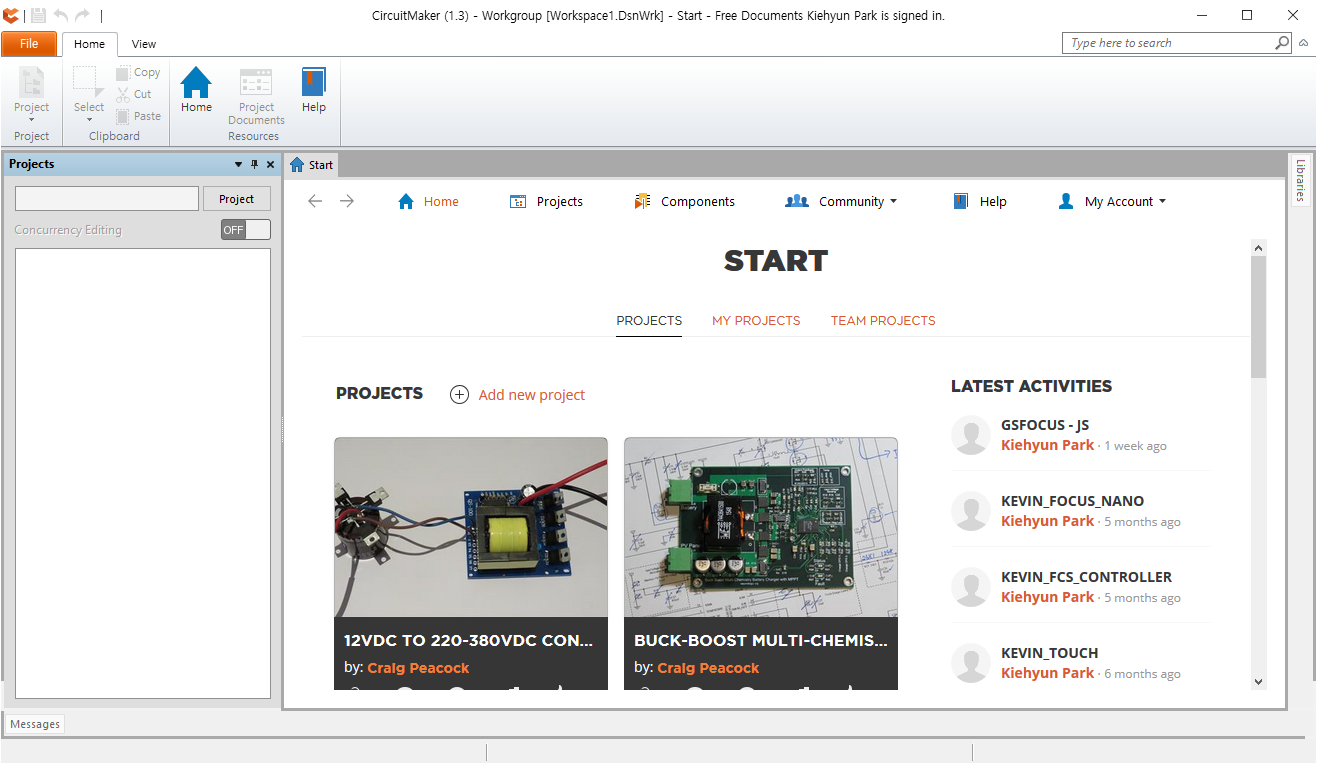
\includegraphics[width=0.56\linewidth]{circuit_maker} 
		};
		\draw (0.3, 5.6) node {(a)};
		\draw (7.3, 5.6) node {(b)};
		\end{tikzpicture}
	\end{center}
	\caption{(a) Circuit maker 공식 사이트와 (b) 실행 화면.}
	\label{fig:circuit_maker}
\end{figure}

Fig. \ref{fig:circuit_maker}\는 Circuit maker를 실행한 화면을 나타낸 것이다. Circuit maker 사용법은 유투브 강좌를 통해 익혔다. Circuit maker 사용법을 익히는데 숙지하는 데 오랜 시간이 걸렸기 때문에, 그 사이에 진행된 연구에서는 Fig. \ref{fig:prototype}의 프로토 타입 하드웨어를 이용하여 펌웨어 개발을 수행하였다. Circuit maker로 하나의 PCB를 완성하기까지 다음의 과정을 거치게 된다.

1. 원하는 기능과 모양의 부품을 선택한다.

2. 부품들 사이에 배선을 하여 회로도를 완성한다.

3. 배선에 이상이 없으면 컴파일 과정을 거쳐 PCB에 부품을 배치한다. 

4. 배치된 부품들 간에 실제 라우팅 (routing) 과정으로 배선을 연결한다. 

5. 모든 작업이 완료되면 거버 포멧 (gerber format)으로 저장하여 업체에 제작을 의뢰한다.

제작한 PCB는 총 3가지 종류가 있는데, Fig. \ref{fig:Schematic_Prints}\는 최종 완성한 기판의 회로도이며, Fig. \ref{fig:pcb}\은 서킷 메이커로 디자인한 PCB의 삼차원 모습을 나타낸다.

\begin{figure}[h]
	\begin{center}
		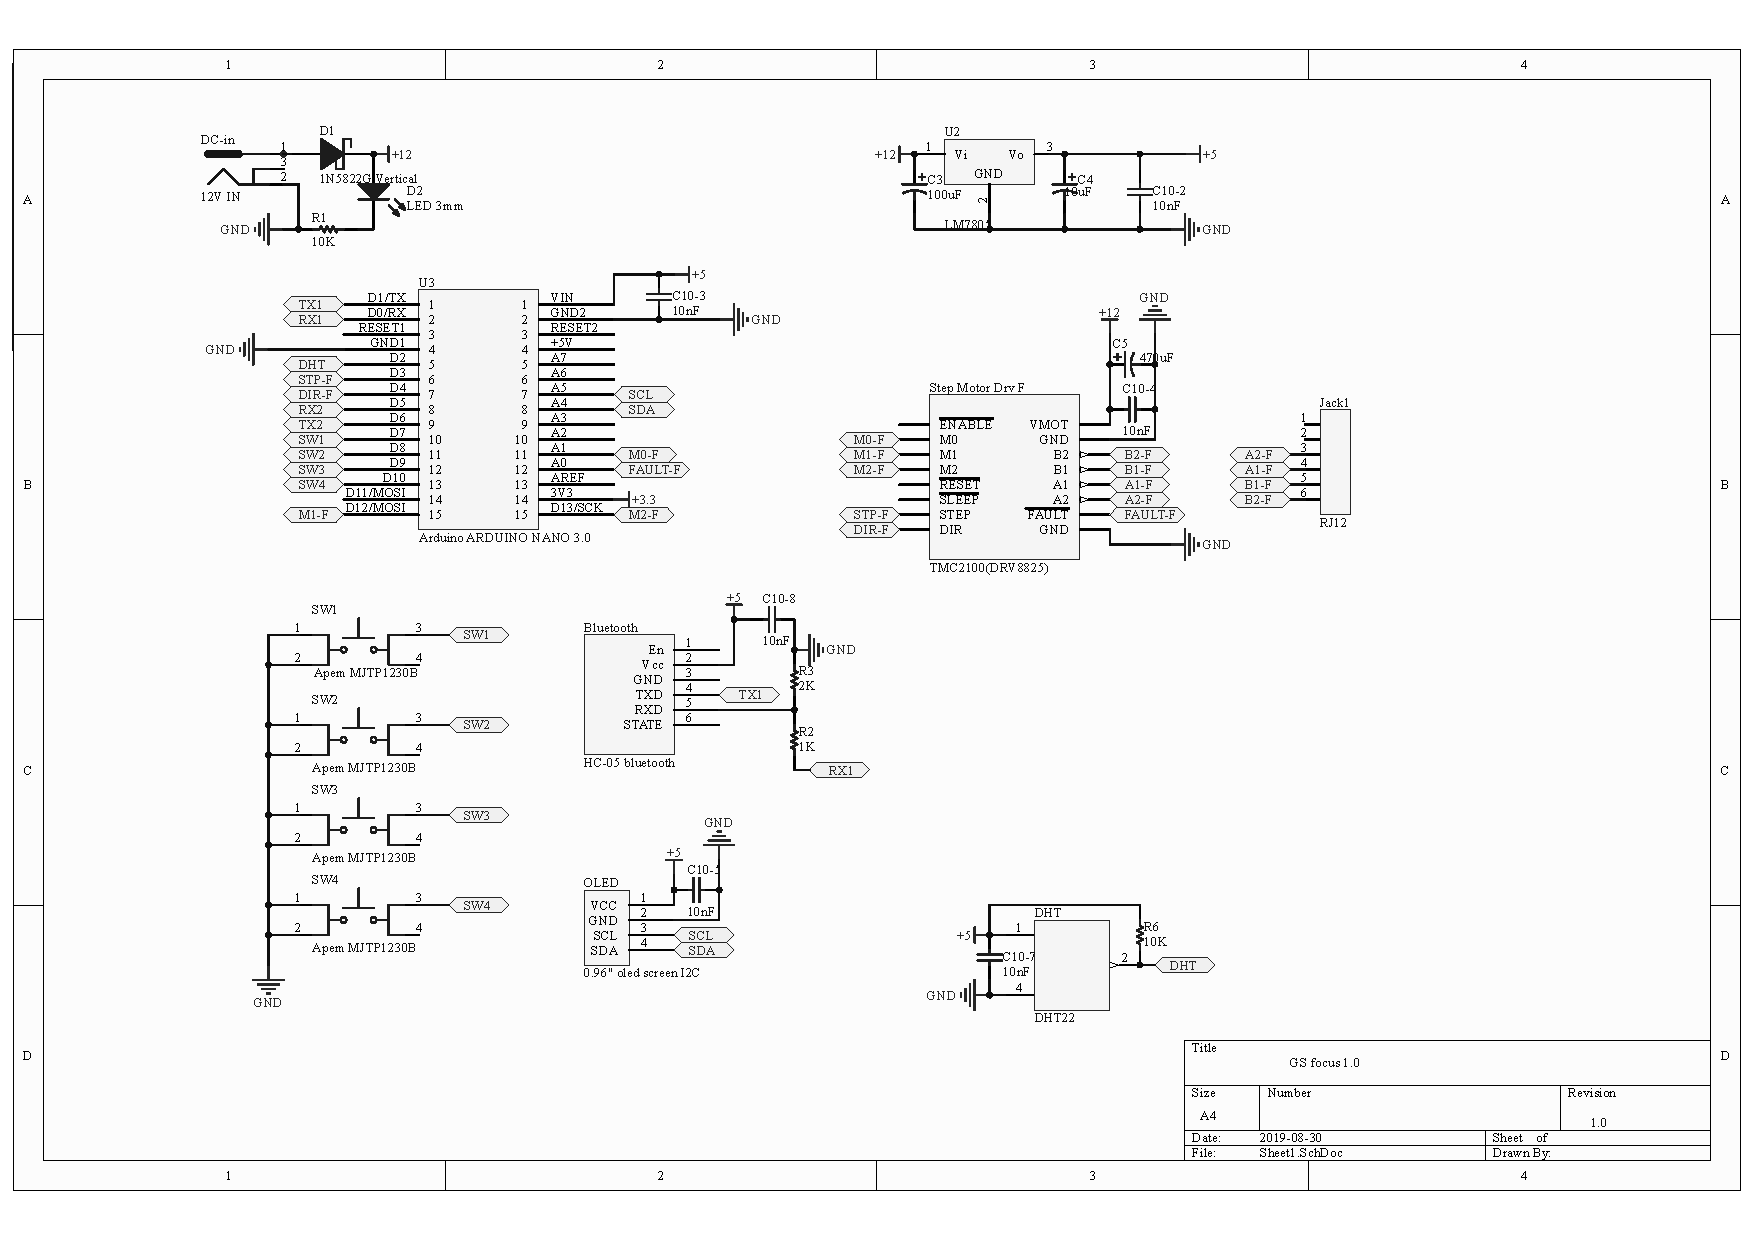
\includegraphics[width=0.75\linewidth]{Schematic_Prints_color}
		\caption{Circuit maker로 작성한 회로}
		\label{fig:Schematic_Prints}
	\end{center}
\end{figure}

\begin{figure}[h]
	\begin{center}
		\begin{tikzpicture}
		\node[anchor=south west, inner sep=0] at (0,0) 
		{
		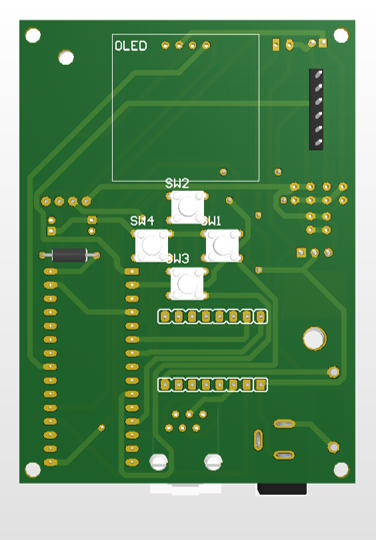
\includegraphics[width=0.35\linewidth]{pcbfront_3d}  
		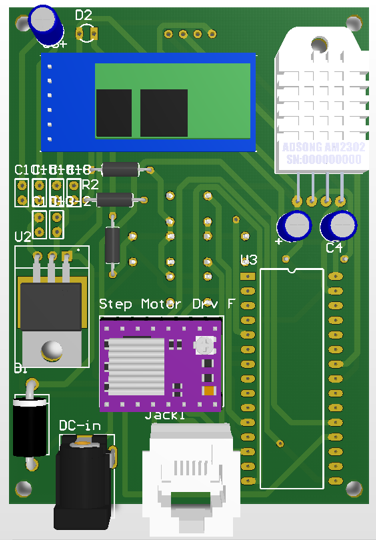
\includegraphics[width=0.34\linewidth]{pcbback_3d}
		};
		\draw (0.1, 8.2) node {(a)};  
		\draw (6.5, 8.2) node {(b)};
		\end{tikzpicture}
	\end{center}
		\caption{Circuit maker로 디자인한 PCB (a) 앞면, (b) 뒷면}
	\label{fig:pcb}
\end{figure}

\clearpage

Fig. \ref{fig:pcbcircuit}\은 처음 제작한 PCB Ver. 1.0\과 개선된 Ver. 1.1\이다. Ver. 1.0\은 크기가 너무 크게 제작되어 Ver. 1.2에서 부품의 배치를 달리하여 크기를 줄여 보았다.

\begin{figure}[h]
	\begin{center}
		\begin{tikzpicture}
		\node[anchor=south west,inner sep=0] at (0,0) 
		{
			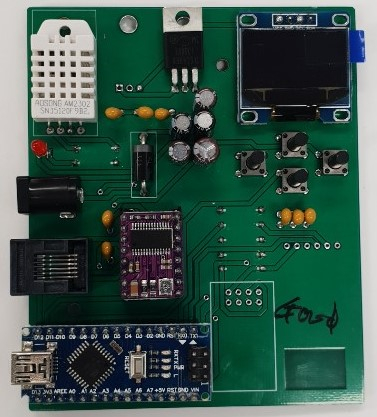
\includegraphics[width=0.362\linewidth]{pcbcircuit}
			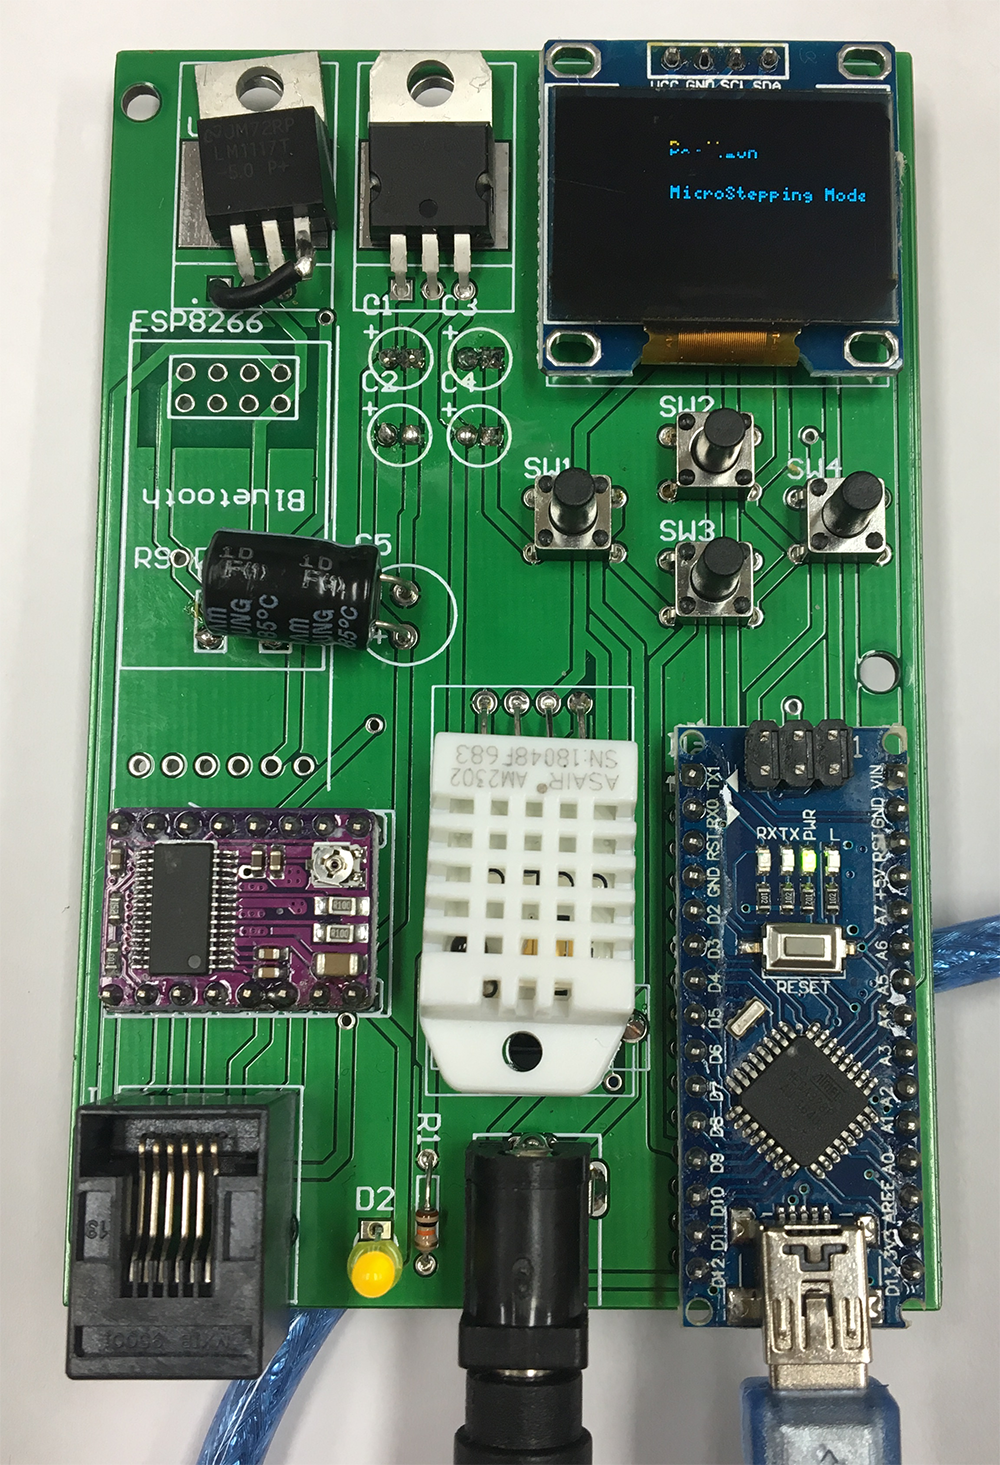
\includegraphics[width=0.272\linewidth]{pcbcircuit-12}
			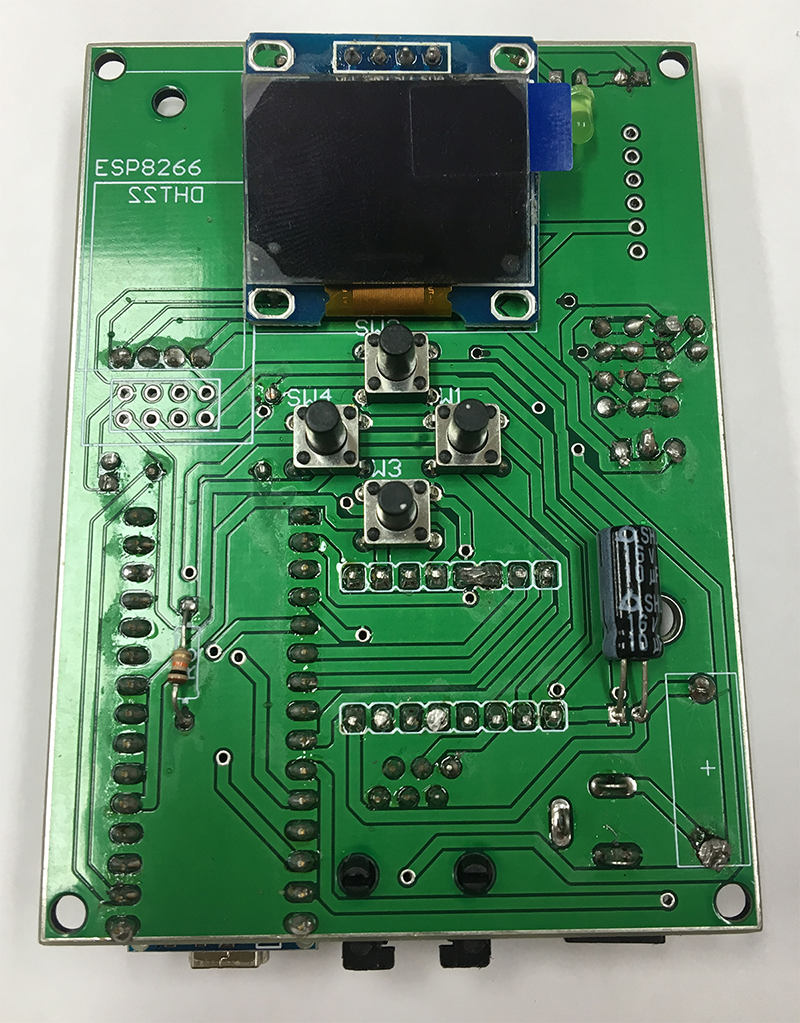
\includegraphics[width=0.313\linewidth]{pcbcircuit-13}
		};
		\draw (0.2, 6.4) node {(a)};
		\draw (6.3, 6.4) node {(b)};
		\draw (11.1, 6.4) node {(c)};
		\end{tikzpicture}
		\caption{제작한 PCB (a) Ver. 1.0, (b) Ver. 1.1, (c) Ver. 1.2.}
		\label{fig:pcbcircuit}
	\end{center}
\end{figure}

\subsubsection{엔클로저(encloser) 제작}

Autodesk 사의 Fusion 360 (https://www.autodesk.com/products/fusion-360/) 을 이용하여 전용 엔클로져를 디자인하였고 그 모습은 Fig. \ref{fig:stl}\와 같다. 디자인한 엔틀로저를 stl (stereolithography) 파일 포멧으로 저장한 후에 3D 프린터 출력하여 저렴하게 하드웨어의 엔클로저를 만들었다. 아ㄱ직갯개선할 부분들이 많지만 엔클로저를 직접 디자인 할 수 있으므로 얼마든지 개선이 가능하다. 

\begin{figure}[h]
	\begin{center}
		\begin{tikzpicture}
		\node[anchor=south west,inner sep=0] at (0,0) 
		{
			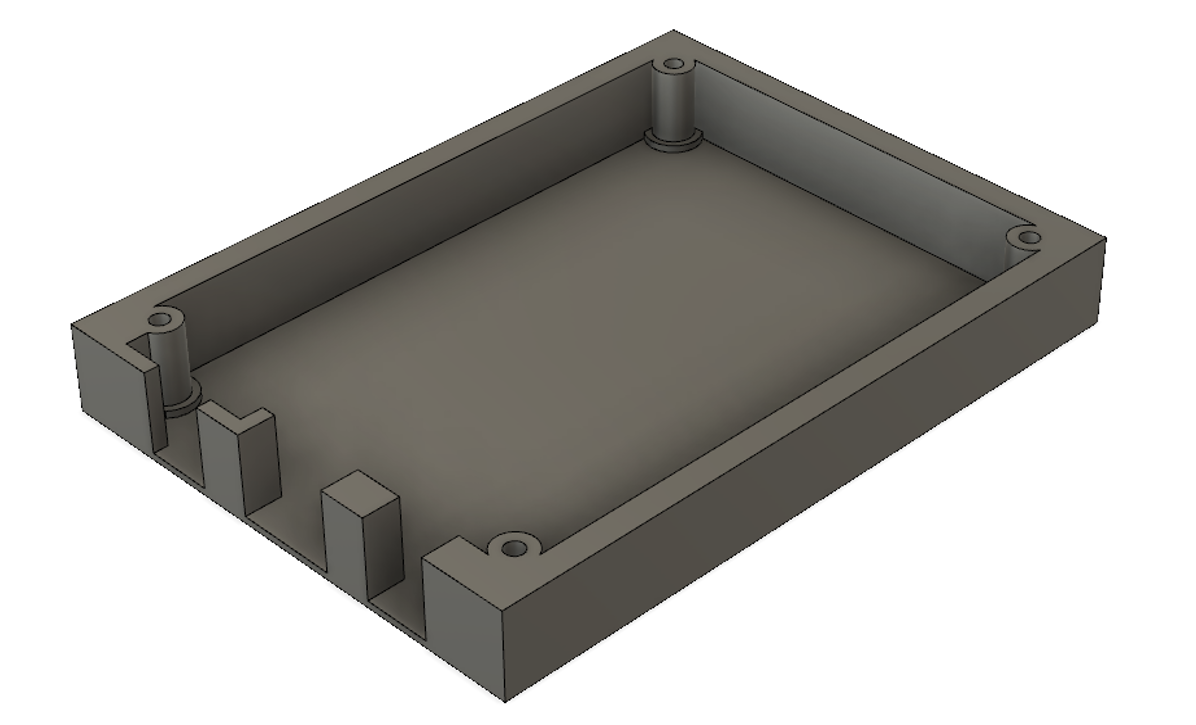
\includegraphics[width=0.5\linewidth]{stldown}
			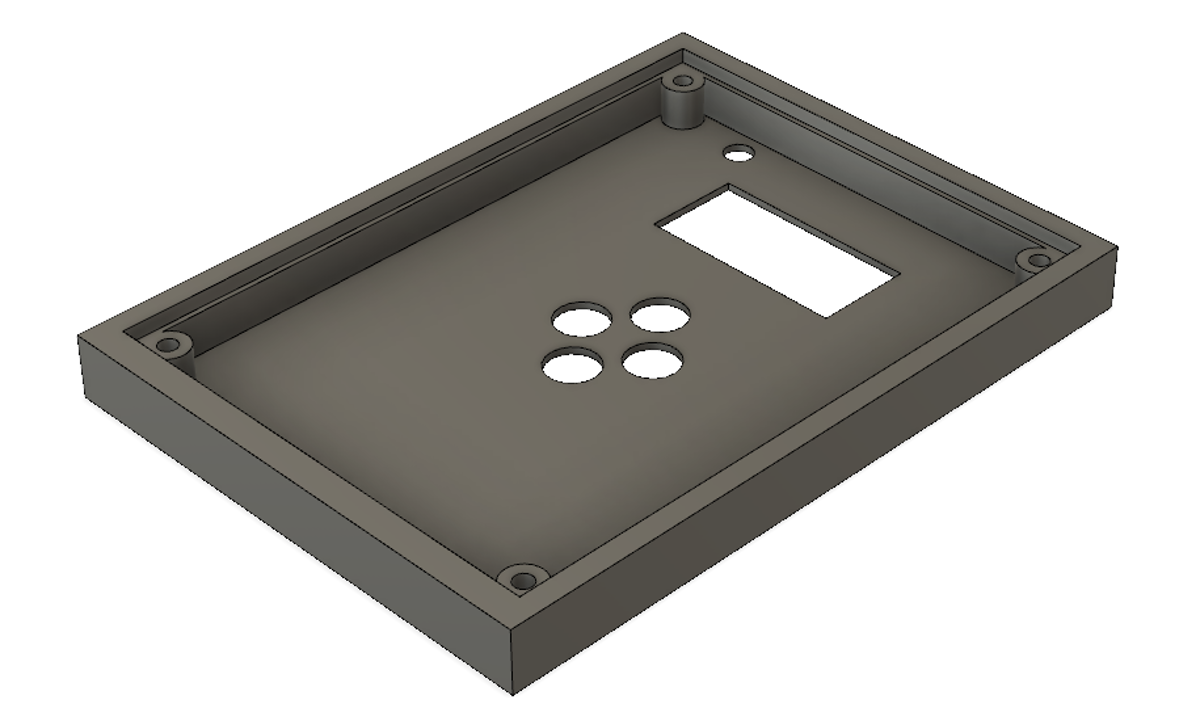
\includegraphics[width=0.5\linewidth]{stlup}
		};
		\draw (0.5, 4.8) node {(a)};
		\draw (8.5, 4.8) node {(b)};
		\end{tikzpicture}
			\caption{Fusion 360으로 디자인한 엔클로저 모습}
		\label{fig:stl}
	\end{center}
\end{figure}

\clearpage

\subsection{펌웨어(firmware) 개발}

펌웨어란 아두이노에 저장되어 MCU를 통해 하드웨어를 제어하는 프로그램이다. GS-touch는 이 펌웨어에 의해 구동되는 것이며 본 연구의 핵심이라고 할수 있다. 펌웨어 개발은 아두이노 IDE\를 이용하였으며 여러 라이브러리를 이용하였다. 또한 추후 개발할 ASCOM driver를 호환성을 고려하여 여러 번의 수정 과정을 거쳐 완성하였으며, 본 연구에서 가장 오랜 시간이 걸린 부분이다. 

\subsubsection{아두이노 라이브러리}
펌웨어에 필요한 기본적인 기능들을 구현하기 위해서는 연결되어있는 부품들을 컨트롤할 수 있는 방법이 필요했고, 이들을 단순화시켜 함수로 정리한 라이브러리를 사용하여 효율적으로 개발을 진행할 수 있었다.
IDE에서 새로운 라이브러리를 추가하기 위해서는 상단의 도구 창에서 스케치>라이브러리 포함하기>라이브러리 관리 또는 .ZIP 라이브러리 추가...를 선택하여 관련 작업을 진행할 수 있다.

본 연구에서 사용한 라이브러리는 다음과 같다. 
\begin{description}[font=$\bullet$~\normalfont\scshape\color{red!50!black}]
	\item [AccelStepper.h] 모터의 전반적인 움직임에 있어 필요한 라이브러리다. 스테핑모터를 컨트롤할 수 있도록 하는 기능을 포함하며, 모터의 객체를 생성할 때 스테핑모터 드라이버가 없는 경우는 각각의 핀을 아두이노와 연결하여 객체를 만들 수 있도록 하며, 본 연구와 같이 스테핑모터 드라이버가 있는 경우에는 드라이버의 DIR핀과 STEP핀만을 이용하여 객체를 생성할 수도 있다. 중요한 함수들을 몇가지 나열하자면, 
	
	AccelStepper::currentPosition() : 현재 position에 있는 값을 반환한다.\\
	AccelStepper::setCurrentPosition(int p) : p를 현재 position으로 한다.\\
	AccelStepper::moveTo(int p) : p위치의 position으로 이동한다.
	
	등이 존재한다. AccelStepper.h 라이브러리의 단점은 그 자체로 microstepping을 지원하지 않기 때문에 이를 바꾸기 위해서는 드라이버를 통해 강제로 바꾸어야하며, 이로 인해 바뀌는 step당 position을 적용시키기 어렵기 때문에 microstepping을 변환하기 위해서는 setCurrentPosition함수가 반드시 동반되어야 한다는 점이다.
	
	\item [DHT.h] DHT22의 컨트롤을 가능하게 하는 라이브러리다. DHT22는 하나의 핀으로 입력과 출력을 모두 하기 때문에 그 방법과 순서만 알면 비교적 쉽게 함수가 제작이 가능하다. DHT22로 온도와 습도를 입력받을 때 걸리는 시간(약 2초당 한번)을 계산하여 펌웨어를 개발하는 것이 좋다.
	
	\item [Adafruit\_SSD1306.h] 본 연구에서 사용된 OLED인 SSD1306을 컨트롤하기 위해 필요한 라이브러리로, 보통 Adafruit\_GFX.h와 Wire.h를 함께 사용하게 된다. SSD1306은 I2C 통신을 사용하므로 복잡한 통신을 이용하기 위해서는 다른 라이브러리들 또한 포함시켜야 할 것이다. 이 라이브러리는 업로드 속도가 빠르고 한번에 모든 화면을 바꿀 수 있다는 장점이 있지만, 사용할 수 있는 폰트가 정해져 있고 아두이노의 자체 메모리를 아주 많이 잡아먹는다는 단점이 있다.
	
	\item [U8glib.h] 많은 종류의 OLED를 컨트롤할 수 있도록 개발된 라이브러리로, 지원하는 OLED 중 SSD1306또한 포함되어 있다. Adafruit\_SSD1306.h와는 다르게 지원하는 폰트와 그 크기가 비교적 자유로우며, 아두이노의 자체 메모리를 작게 잡아먹으며 한번에 작성하지 않는다는 특징이 있지만 업로드 시 많은 시간이 소요된다는 단점도 존재한다.
\end{description}

\subsubsection{serialPort 통신}
펌웨어를 개발할 때 필요한 중요한 기능 중 하나는 컴퓨터와 통신이 가능해야 한다는 것이다. 아두이노는 UART 시리얼 통신을 사용하는 데, 직렬 통신을 사용하기 때문에 그 속도는 떨어질 수 있어도 더 먼 거리를 보낼 수 있다는 장점이 있으며, UART방식을 사용하기 때문에 정해진 BaudRate로만 통신이 가능하다. 아두이노의 0번 핀(RX: Receive Data)이 컴퓨터에서 보내는 신호를 받고, 1번 핀(TX: Transmit Data)으로 신호를 보내게 되며, 이들은 USB 케이블을 통해 컴퓨터와 직접적으로 연결된다.

아두이노 IDE 상에서는 우측 상단의 돋보기 모양의 아이콘을 클릭함으로써 시리얼 모니터를 실행할 수 있다. 시리얼 통신을 이용하기 위해서는 지정된 BaudRate로 COM Port를 열어야한다. 따라서 코드 중에 반드시 시리얼 포트를 여는 코드가 있어야 하며, 이후 수신된 값을 활용할 수 있는 기법들을 이용해 데이터를 사용할 수 있도록 한다. 주로 사용되는 함수는 다음과 같다.

\begin{description}[font=$\bullet$~\normalfont\scshape\color{red!50!black}]
	\item [Serial.begin(int BaudRate)] 지정된 BaudRate로 시리얼 통신을 시작한다.
	\item [Serial.print(String s)] String형 변수 s의 값을 컴퓨터로 송신한다. 비슷한 함수로 Serial.println(String s)가 있는 데, 이는 값을 수신한 이후 줄을 띄게 한다.
	\item [Serial.available()] 시리얼 통신이 진행되고 있는지를 bool 형태로 반환한다. 이를 응용하면 다음과 같은 예제로 수신된 String을 미리 선언된 inputString에 저장할 수 있다.
	%%P_serialEvent사진 첨부
\end{description}


\subsection{ASCOM driver 및 컨트롤 프로그램 개발}

ASCOM standard는 망원경을 움직이기 위하여 지원하는 시스템 중 하나로, 현재 제작되고 사용되는 많은 망원경들이 ASCOM standard를 따르고 있기 때문에 이를 사용하여 망원경을 움직이는 프로그램을 만들게 되면 여러 망원경에도 같이 사용할 수 있게 되어 호환성에 있어 큰 이점을 가지게 된다. 이것이 가능한 이유는 ASCOM standard 만의 프로토콜(protocol)이 존재하기 때문인데, 드리아버를 사용하여 이를 펌웨어와 연결시켜 통신을 할 때, ASCOM standard protocol을 사용하면 펌웨어와의 통신이 원활하게 이루어질 수 있게 되고, 다른 드라이버와도 연결할 수 있게 만들 수 있게 된다.

ASCOM은 Visual Studio를 이용한 여러 가지 예제나 개발 환경을 제공하는데, developer 버전을 제공하여 아이콘이나, 실행 배경 등 Visual Studio를 이용한 ASCOM 드라이버의 개발에 필요한 여러 작업 환경들을 지원고 있어 ASCOM driver는 Visual Studio를 사용하여 개발하였다. Visual Studio는 Microsoft에서 제공하는 통합 개발 환경으로, Visual Basic, Visual C\# 등 여러 가지 언어를 제공하며, Windows .NET환경에서 개발을 진행할 수 있다는 큰 장점이 있다. 본 드라이버의 언어 또한 Windows. NET을 기반으로 하고 있으므로 Windows. NET 기반의 개발 환경을 제공하는 Visual Studio를 사용하여 개발할 수 있었다. 추후 개발이 원활하게 진행되면, MFC 라이브러리를 이용한 드라이버의 개발을 진행하여 개발의 직관성을 더 높일 수도 있을 것이며, MFC 라이브러리를 이용하며 만든 드라이버 또한 Visual Studio를 통한 원활한 개발이 가능하다. 이를 위해서는 C\#으로 개발된 프로그램을 regasm.exe로 활성화시킬 필요가 있다.

\subsubsection{드라이버 파일 생성 및 설정}
기본적으로 ASCOM에서는 개발자들을 위한 Platform 6 Developer Components를 지원하게 된다. 사이트에서 직접 다운로드 받을 수 있는 파일 속에는 C\# 형식으로 들어있는 Driver.cs와 SetupDialogForm.cs를 지원하여 ASCOM과 미리 연결할 수 있도록 할 뿐만이 아니라 아이콘과 라이센스 등 개발 시 주의점이나 필요한 요소들을 지원해준다.

개발을 C\#의 형태로 진행하므로 이를 구동시키기 위한 Visual Studio로 대부분의 개발이 진행된다. Visual Studio에서 C\#을 구동할 수 있게 만드는 Visual C\#을 다운로드 받은 뒤, ASCOM Device Driver까지 다운받았다면 ...과 같은 방법을 통해 ASCOM Device Driver 파일을 생성하여 개발을 진행한다. 최초로 생성되어 있는 파일은 Driver.cs와 SetupDialogForm.cs이며, 이후 파일들은 프로젝트에 파일을 생성하는 방법으로 추가가 가능하다.

C\#만으로 개발을 진행할 경우 빌드에 성공했을 시에 release에 여러 dll파일들이 남게 된다. 간혹 빌드 실패라고 하면서 어셈블리를 형식 라이브러리(ASCOM Driver은 형식 라이브러리이다)로 변환하지 못한 경우가 있는 데, MFC(Windows 운영체제의 GUI 프로그램을  C++을 활용하여 할 수 있게 해주는 함수라이브러리)를 활용하지 않는 경우에는 무시해도 상관없다. 혹은 Visual Studio를 관리자로 실행하지 않아 컴파일되지 않는 경우또한 존재한다.

그외에 regasm.exe를 사용하여 COM Interop에 등록하여야 하는 경우가 있는데, 프로그램의 자체 속성>빌드>COM Interop 등록 박스를 체크한 뒤에 도구>GUID 만들기>5번을 이용하여 형식에 맞게 Assembly.cs파일에 바꾸어주면 오류가 해결된다.

\subsubsection{dll 파일 출력 및 setup파일 생성}
드라이버를 32bit 환경에서 사용하는지, 혹은 64bit 환경에서 사용하는지에 따라 변경되어야 할 요소들이 존재한다. 본 연구에서는 MaximDL이 32bit 환경의 드라이버만 실행할 수 있으므로 32bit를 기본으로 개발하였다. 이를 바꾸기 위해서는 구성 관리자>구성을 Release로 바꾸고, 사용하는 환경에 따라서 '활성 솔루션 플랫폼'과 '플랫폼'을 x86과 x64로 '새로 만들기'를 이용하여 설정하면 된다.

%%http://www.jrsoftware.org/isinfo.php inno setup 홈페이지
setup.exe 파일을 생성하기 위해서는 setup파일을 생성할 수 있는 프로그램이 필요하다. 본 연구에서는 'inno setup'이라는 프로그램을 사용하였으며, ASCOM Developer Components>Installer Generator>Resources에 들어있는 DriverInstallTemplate.iss파일을 참고하여 inno setup 파일을 생성 후 실행파일에 (bin>x86>Release 혹은 bin>x64>Release 파일 속에 있는) ASCOM.(드라이버 이름).Focuser.dll으로 설정한 뒤 컴파일을 진행하면 setup파일을 통해 ASCOM에 드라이버를 등록하여 사용할 수 있다.